\documentclass[t,10pt,fleqn]{beamer}

%%% My preferred theme choices.  More information is available at
%
%  https://en.wikipedia.org/wiki/Beamer_(LaTeX)
%  http://mirrors.ctan.org/macros/latex/contrib/beamer/doc/beameruserguide.pdf

\usetheme{Malmoe}
\usecolortheme{rose}
\useinnertheme{rounded}
\useoutertheme[subsection=false,footline=authorinstitute]{miniframes}
\usenavigationsymbolstemplate{}

%%% The following command inserts a slide with the outline at the
%%% beginning of each section, highlighting the current section.  It
%%% is optional.

\AtBeginSection[]
{
	\begin{frame}{Outline}
		\tableofcontents[currentsection]
	\end{frame}
}

\newenvironment{amatrix}[1]{%
	\left(\begin{array}{@{}*{#1}{r}|r@{}}
}{%
	\end{array}\right)
}

\newenvironment{bulletlist}
	 {
			\begin{list}
				 {$\bullet$}
%         {$\cdot$}
				 {
						\setlength{\itemsep}{.5ex}
						\setlength{\parsep}{0ex}
						\setlength{\leftmargin}{1.5 em}
						\setlength{\rightmargin}{0.5em}
						\setlength{\parskip}{0ex}
						\setlength{\topsep}{0ex}
				 }
	 }
	 {
			\end{list}
	 }


\newcount\arrowcount
\newcommand\arrows[1]{
				\global\arrowcount#1
				\ifnum\arrowcount>0
								\begin{matrix}
								\expandafter\nextarrow
				\fi
}

\newcommand\nextarrow[1]{
				\global\advance\arrowcount-1
				\ifx\relax#1\relax\else \xrightarrow{#1}\fi
				\ifnum\arrowcount=0
								\end{matrix}
				\else
								\\
								\expandafter\nextarrow
				\fi
}


%%% It is sometimes easier to have graphics in a subfolder (or
%%% subfolders) of the current folder, in this case that folder is
%%% called Figures
\graphicspath{ 
	{../Figures/}{../Images/}
}


\usepackage{multicol}
	\usepackage{booktabs}
	\usepackage{amsmath}
\usepackage{epsfig}
\usepackage{enumerate}
\usepackage{graphicx}

\def\ds{\displaystyle}
\def\u{{\mathbf u}}
\def\v{{\mathbf v}}
\def\w{{\mathbf w}}

\def\A{{\mathbf A}}



\def\B{{\mathbf B}}
\def\C{{\mathbf C}}
\def\D{{\mathbf D}}
\def\E{{\mathbf E}}
\def\X{{\mathbf X}}
\def\U{{\mathbf U}}

\def\T{{\mathbf T}}

\def\det{\text{det}}
\def\row{\text{row}}
\def\col{\text{col}}
\def\dim{\text{dim}}
\def\span{\text{span}}
\def\rank{\text{rank}}
\def\dom{\text{dom}}
\def\domain{\text{domain}}
\def\range{\text{range}}
\def\RREF{\text{RREF}}
\def\null{\text{null}}
\def\nullity{\text{nullity}}
\def\ker{\text{ker}}


\def\e{{\mathbf e}}
\def\x{{\mathbf x}}
\def\y{{\mathbf y}}
\def\b{{\mathbf b}}
\def\c{{\mathbf c}}

\def\r{{\mathbf r}}

\def\0{{\mathbf 0}}
\def\v{{\mathbf v}}
\def\I{{\mathbf I}}


\def\AA{\mathcal{A}}
\def\R{\mathcal{R}}

\def\S{\mathcal{S}}

\def\V{\mathcal{V}}

\def\M{\mathcal{M}}

\def\({\biggr ( }
\def\){\biggr ) }

\def\[{\biggr [ }
\def\]{\biggr ] }

\def\d{\partial}

\newcommand{\tu}[1]{\underline{\textit{#1}}}

% This is the main file
% This is the main file

\title[DDCPM]%
			{A Data-driven Comparison of Plague Models}
\subtitle{Senior Project}
\author[Luke Mattfeld]{Luke Mattfeld}
\institute[EWU]{Eastern Washington University}
\date{Fall, 2020}

\begin{document}

\begin{frame}
	\titlepage

\end{frame}
%-------------------------------------------------------------------------------------------------------------------------------------
%-------------------------------------------------------------------------------------------------------------------------------------
\section{Background}
%------------------------------------------------------------------------------------------------------------------------------
\begin{frame}{The Plague}
	\vspace{-.3cm}
	\begin{block}{Which Plague?}
		\begin{columns}
			\begin{column}{0.40\textwidth}
				\begin{itemize}
					%					\pause
					\item Names: The Black Death, Bubonic Plague, etc.
					      \pause
					      \begin{itemize}
						      \pause
						      \item Bubonic plague
						            \pause
						      \item Pneumonic plague
						            \pause
						      \item Septicemic plague
						            \pause
						            \\
					      \end{itemize}
					\item Bacteria behind it all: Yersinia pestis
					      \\
				\end{itemize}
			\end{column}
			\begin{column}{0.55\textwidth}
				\onslide
				\begin{figure}
					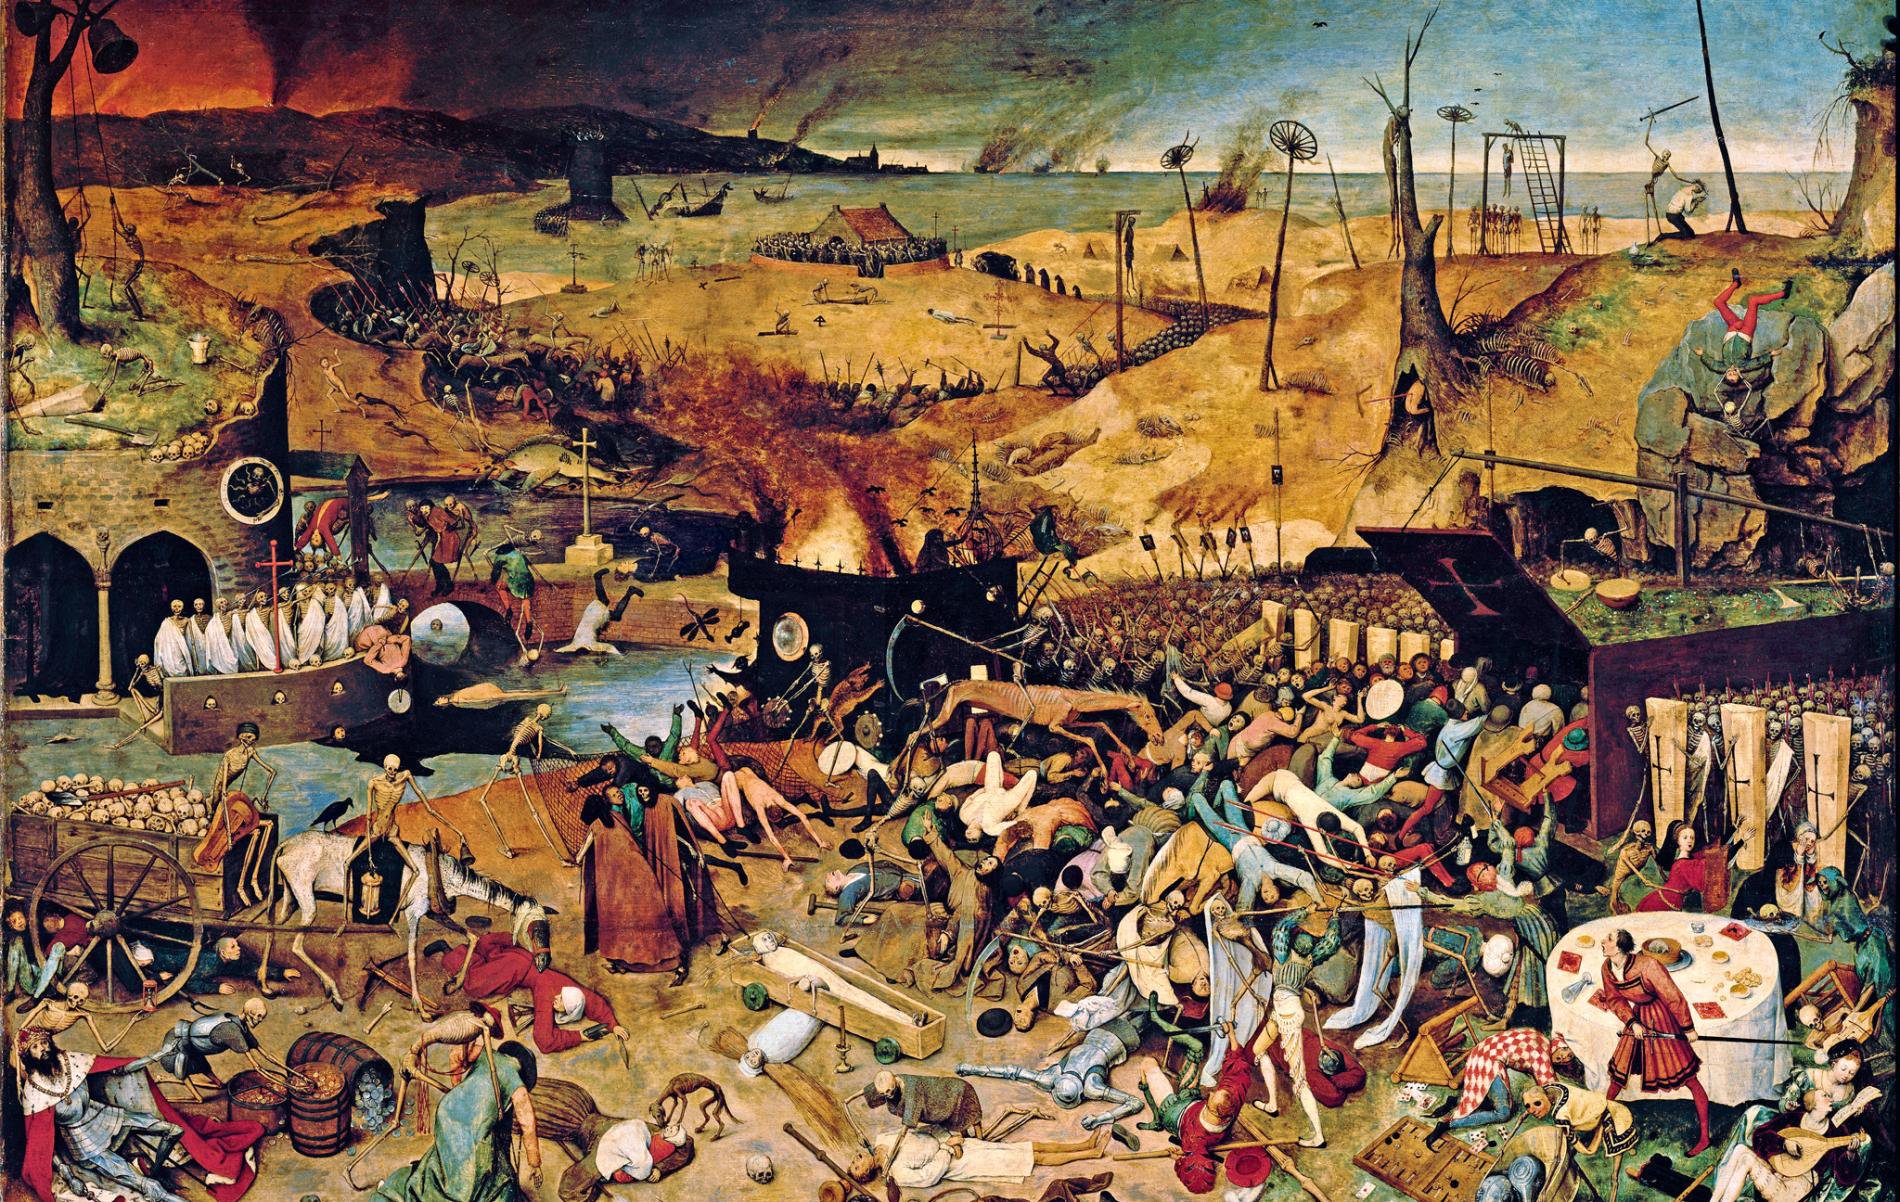
\includegraphics[width=\linewidth]{triumph-of-death.jpg}
					\caption{"The Triumph of Death" - Pieter Bruegel the Elder - 1562}
				\end{figure}
			\end{column}
		\end{columns}
	\end{block}
\end{frame}

\begin{frame}{The Plague}
	\vspace{-.3cm}
	\begin{block}{How it Spread}
		\begin{itemize}
			\pause
			\item Aspirated \pause $\rightarrow$ Pneumonic model
			      \pause
			\item Rats to Fleas to Humans \pause $\rightarrow$ Rat-Flea transmission (RFT) model
			      \pause
			\item Other \pause $\rightarrow$ Human-Ectoparasite model (Dean et al.)
			      \pause
			\item New RFT Model \pause $\rightarrow$ Lynch-Oster RFT model
		\end{itemize}
	\end{block}
	\pause
	\begin{block}{Goal}
		\begin{itemize}
			\pause
			\item Use data on plague spread to compare proposed models \pause
			\item Get indication of spread type per data
		\end{itemize}
	\end{block}
\end{frame}

%\begin{frame}{Plague}
%	\vspace{-.3cm}
%	
%	\pause
%\end{frame}


%-------------------------------------------------------------------------------------------------------------------------------------
%-------------------------------------------------------------------------------------------------------------------------------------
\section{Preliminary Models}
%------------------------------------------------------------------------------------------------------------------------------
\begin{frame}{Pneumonic Model}
	\vspace{-.3cm}
	\begin{block}{Humans - SID}
		$$\frac{dS_h}{dt} = - \beta_p \frac{S_h I_h}{N_h}$$

		$$\frac{dI_h}{dt} = \beta_p \frac{S_h I_h}{N_h} - \gamma_p I_h$$

		$$\frac{dD_h}{dt} = \gamma_p I_h$$
		\only<+>{\center \includegraphics[width=0.65\linewidth]{sid-graph}}
		\only<+->{
			\begin{itemize}
				\item SID model
				      %			      \pause
				\item $S_h$ - Susceptible, $I_h$ - Infected, $D_h$ - Deaths, $N_h$ - Total Population
				      %			      \pause
				\item $\beta_p$ - Transmission rate, $\gamma^{-1}$ - Infectious period
			\end{itemize}
		}
	\end{block}
	%	\pause
\end{frame}

\begin{frame}{Keeling-Gilligan Rat Model}
	\vspace{-.3cm}
	\begin{block}{Fleas}
		$$\frac{dH}{dt} = r_f H \left( 1 - \frac{H}{K_f} \right)$$
		$$\frac{dF}{dt} = (1 - g_r) \gamma_r I_r H - d_f F$$
		\begin{itemize}
			\item H - Number of fleas per rat
			\item F - Number of infected fleas not on rats
		\end{itemize}
	\end{block}
	\pause
\end{frame}

\begin{frame}{Keeling-Gilligan RFT Model}
	\vspace{-.3cm}
	\begin{block}{SIRD - Rats \& Humans}
		$$\frac{dS_j}{dt} = - \beta_r \frac{S_j F}{N_j} \left[ 1 - e^{-aN_r} \right]$$
		$$\frac{dI_j}{dt} = \beta_r \frac{S_j F}{N_j} \left[ 1 - e^{-aN_r} \right] - \gamma_j I_j$$
		$$\frac{dR_j}{dt} = g_j \gamma_j I_j$$
		$$\frac{dD_j}{dt} = (1 - g_j) \gamma_j I_j$$
		\only<+>{\center \includegraphics[width=0.65\linewidth]{sird-graph}}
		\only<+->{
			\begin{itemize}
				\item SIRD model where j = Rats, Fleas
				      %			      \pause
				\item $S_j$ - Susceptible, $I_j$ - Infected, $R_j$ - Recovered, $D_j$ - Dead, $N_j$ - Total Population
				      %			      \pause
			\end{itemize}
		}
	\end{block}
\end{frame}

% Human-Ecto Model
\begin{frame}{Human-Ectoparasite Model}
	\vspace{-.3cm}
	\begin{block}{Parasites - SI}
		$$\frac{dS_L}{dt} = r_L S_L \left( 1 - \frac{N_L}{K_L} \right) - \left[ \left( \beta_{low} I_{low} + \beta_{high} I_{high} \right) \frac{S_L}{N_h} \right]$$
		$$\frac{dI_L}{dt} = \left[ \left( \beta_{low} I_{low} + \beta_{high} I_{high} \right) \frac{S_L}{N_h} \right] - \gamma_L I_L$$
		\only<+>{\center \includegraphics[width=0.45\linewidth]{si-graph}}
		\only<+->{
			\begin{itemize}
				\item SI Model
				\item $S_L$ - Susceptible, $I_L$ - Infected
				\item $\gamma_L^{-1}$ - Avg. infectious period, $r_L$ - Intrinsic growth rate, $K_L$ - Lice carrying capacity
			\end{itemize}
		}
	\end{block}
\end{frame}

\begin{frame}{Human-Ectoparasite Model}
	\vspace{-.3cm}
	\begin{block}{Humans - SIIRD}
		$$\frac{dS_h}{dt} = -\beta_L \frac{S_h I_L}{N_h}$$
		$$\frac{dI_{low}}{dt} = \beta_L \frac{S_h I_L}{N_h} - \sigma_b I_{low}$$
		$$\frac{dI_{high}}{dt} = (1-g_h) \sigma_b I_{low} - \gamma_b I_{high}$$
		$$\frac{dR_h}{dt} = g_h \sigma_b I_{low}$$
		$$\frac{dD_h}{dt} = \gamma_b I_{high}$$
		\only<+>{\center \includegraphics[width=0.55\linewidth]{siird-graph}}
		\only<+->{
			\begin{itemize}
				\item $SI_LI_hRD$ Model
				\item $S_h$ - Susceptible, $I_{low}$ - Infected (low level), $I_{high}$ - Infected (high level), $R_h$ - Recovered, $D_h$ - Dead
			\end{itemize}
		}
	\end{block}
\end{frame}

% Rat-Flea-Transmission 2
\begin{frame}{Lynch-Oster RFT Model}
	\vspace{-.3cm}
	\begin{block}{Rats \& Fleas - Logistic}
		$$\frac{dR_T}{dt} = (\frac{\beta_R}{K_R})R_T(K_R-R_T)-\delta R_c$$
		$$\frac{dR_c}{dt} = \alpha \frac{F_c}{F_T} (R_T-R_c)-\frac{\beta_R}{K_R}(R_T)(R_c) - \delta R_c - \gamma R_c$$
		% \hline
		\vspace{0.1cm}
		$$\frac{dF_T}{dt} = (\frac{\beta_F}{K_F})F_T(K_F-F_T)-\rho F_T$$
		$$\frac{dF_c}{dt} = \lambda \frac{R_c}{R_T} (F_T-F_c) - \rho F_c$$
		\begin{itemize}
			\item Logistic Model
			      \pause
			\item T - total, c - Infected
			\item $\beta$ - Intrinsic birth rate, $\mu$ - Intrinsic death rate, $\gamma$ - Rat recovery rate, $\{\rho, \delta\}$ - Plague death rate, $\{\lambda, \alpha\}$ - Plague infectivity, K - Carrying capacity
		\end{itemize}
	\end{block}
	\pause
\end{frame}

\begin{frame}{Lynch-Oster Rat Model}
	\vspace{-.3cm}
	\begin{block}{Humans - SEIR}
		$$\frac{dS}{dt} &= \beta (S+R_b) - \sigma S \frac{F_c}{F_T} - \mu S$$
		$$\frac{dE}{dt} &= \sigma S \frac{F_c}{F_T} - \nu E - \mu E$$
		$$\frac{dI}{dt} &= \nu E - \phi I - rI$$
		$$\frac{dR_b}{dt} &= rI - \mu R_b$$
		$$\frac{dD}{dt} &= \phi I - \mu N_h$$
		\only<+>{\center \includegraphics[width=0.65\linewidth]{seird-graph}}
		\only<+->{
			\vspace{-.3cm}
			\begin{itemize}
				\item SEIR model
				\item $S$ - Susceptible, $E$ - Infected, $I$ - Infected, $R_b$ - Recovered, $D$ - Deaths, $N_h$ - Total Population
				\item $\beta$ - Human birth rate, $\sigma$ - chance of being infected by flea, $\mu$ - Intrinsic death rate, $v^{-1}$ - Incubation period, $r^{-1}$ - Recovery rate, $\phi^{-1}$ - Plague death rate
			\end{itemize}
		}
	\end{block}
\end{frame}



%-------------------------------------------------------------------------------------------------------------------------------------
%-------------------------------------------------------------------------------------------------------------------------------------
\section{Method: MCMC}
%------------------------------------------------------------------------------------------------------------------------------

\begin{frame}{Method}
	\vspace{-.3cm}
	\begin{block}{How to Compare}
		\begin{itemize}
			\pause
			\item Given data and a model, why not just run directly?
			      \pause
			\item Problem: Unknown Parameters
			      \pause
			      \begin{itemize}
				      \item Lack of data
				            \pause
				      \item No way to measure
				            \pause
				      \item Nontrivial to compute
				            \pause
				      \item Changes from case to case
				            \pause
			      \end{itemize}
			\item Solution: Markov-Chain Monte-Carlo
		\end{itemize}
	\end{block}

\end{frame}



\begin{frame}{Method}
	\vspace{-.3cm}
	\begin{block}{Monte Carlo Method}
		\begin{itemize}
			\pause
			\item Have: Unknown distribution from behavior
			      \pause
			\item Want: Distribution information
			      \pause
			      \begin{itemize}
				      \item 1. Simulate the underlying behavior
				            \pause
				      \item 2. Run lots of simulations
				            \pause
				      \item 3. Examine results as number of iterations N $\rightarrow$ Really Big
				            \pause
			      \end{itemize}
			\item Get: Pretty good distribution estimation
		\end{itemize}
	\end{block}
\end{frame}

\begin{frame}{Method}
	\vspace{-.3cm}
	\begin{block}{Markov Chains}
		\begin{itemize}
			\pause
			\item Series (chain) of computed values
			      \pause
			\item Dependent on the previous state
			      \pause
			\item Many uses
			      \pause
			      \begin{itemize}
				      \item Model a state machine
				            \pause
				      \item Train into predictive algorithms
				            \pause
				      \item Explore parameter distribution space
				            \pause
			      \end{itemize}
		\end{itemize}
	\end{block}
\end{frame}

\begin{frame}{Method}
	\vspace{-.3cm}
	\begin{block}{MCMC}
		\begin{itemize}
			\pause
			\item Monte Carlo simulation generated using Markov Chains
			      \pause
			\item Bayesian Statistics
			      \pause
			\item Given:
			      \begin{itemize}
				      \pause
				      \item $\vec{\alpha}$ - vector of unknown parameters
				            \pause
				      \item $\mathcal{D}$ - data
				            \pause
				      \item $\mathcal{M}$ - model
			      \end{itemize}
			      \pause
			\item
			      \only<+>{Want to find: $P(\vec{\alpha} | \mathcal{D}, \mathcal{M})$ \pause}
			      \only<+->{Make use of Bayes Formula:}
		\end{itemize}
		$$ P(\vec{\alpha} | \mathcal{D}, \mathcal{M}) = \frac{P(\mathcal{D} | \vec{\alpha}, \mathcal{M}) P(\vec{\alpha} | \mathcal{M})}{P(\mathcal{D} | \mathcal{M})}$$
		\pause
		%    \vspace{-.3cm}
		\begin{itemize}
			\item Posterior - $P(\vec{\alpha} | \mathcal{D}, \mathcal{M})$
			\item Likelihood - $P(\mathcal{D} | \vec{\alpha}, \mathcal{M})$
			\item Prior - $P(\vec{\alpha} | \mathcal{M})$
		\end{itemize}
		%		\pause
		$$ P(\vec{\alpha} | \mathcal{D}, \mathcal{M}) \propto P(\mathcal{D} | \vec{\alpha}, \mathcal{M}) P(\vec{\alpha} | \mathcal{M})$$

	\end{block}
	\pause
\end{frame}


\begin{frame}{Method}
	\vspace{-.3cm}
	\begin{block}{MCMC Process}
		\centering
		\begin{figure}
			\includegraphics[width=0.9\linewidth]{mcmc-diag-kipping}
			\caption{David Kipping - Sagan 2016 Presentation on MCMC}
		\end{figure}
	\end{block}
\end{frame}

\begin{frame}{Method}
	\vspace{-.3cm}
	\centering
	\begin{block}{MCMC - Metropolis}
		\includegraphics[width=0.65\textwidth]{mcmc-start.png}
	\end{block}
\end{frame}

\begin{frame}{Method}
	\vspace{-.3cm}
	\centering
	\begin{block}{Markov Chains - Metropolis}
		\includegraphics[width=0.65\textwidth]{mcmc-circling.png}
	\end{block}
\end{frame}



%-------------------------------------------------------------------------------------------------------------------------------------
%-------------------------------------------------------------------------------------------------------------------------------------
\section{Comparison}
%------------------------------------------------------------------------------------------------------------------------------

\begin{frame}{Barcelona - 1490}
	\vspace{-.2cm}
	\begin{columns}
		\column{0.5\textwidth}
		\centering
		\includegraphics[width=\linewidth]{pneum/barcelona-40-30-22-15x10}
		\includegraphics[width=\linewidth]{h_ecto/barcelona-40-30-22-15x10}
		\column{0.5\textwidth}
		\centering
		\includegraphics[width=\linewidth]{rats1/barcelona-40-30-22-15x10}
		\includegraphics[width=\linewidth]{rats2/barcelona-40-30-22-15x10}

	\end{columns}
\end{frame}


\begin{frame}{Malta - 1813}
	\vspace{-.2cm}
	\begin{columns}
		\column{0.5\textwidth}
		\centering
		%    Pneumonic Model
		\includegraphics[width=\linewidth]{pneum/malta-40-30-22-15x10}
		%    Keeling-Gilligan Model
		\includegraphics[width=\linewidth]{h_ecto/malta-40-30-22-15x10}
		\column{0.5\textwidth}
		\centering
		%    Human-Ecto Model
		\includegraphics[width=\linewidth]{rats1/malta-40-30-22-15x10}
		%    Lynch-Oster Model
		\includegraphics[width=\linewidth]{rats2/malta-40-30-22-15x10}

	\end{columns}
\end{frame}

\begin{frame}{Florence - 1400}
	\vspace{-.2cm}
	\begin{columns}
		\column{0.5\textwidth}
		\centering
		%    Pneumonic Model
		\includegraphics[width=\linewidth]{pneum/florence-40-30-22-15x10}
		%    Keeling-Gilligan Model
		\includegraphics[width=\linewidth]{h_ecto/florence-40-30-22-15x10}
		\column{0.5\textwidth}
		\centering
		%    Human-Ecto Model
		\includegraphics[width=\linewidth]{rats1/florence-40-30-22-15x10}
		%    Lynch-Oster Model
		\includegraphics[width=\linewidth]{rats2/florence-40-30-22-15x10}

	\end{columns}
\end{frame}


\begin{frame}{Metrics}
	\begin{block}{BIC}
		%\begin{table}[ht]
		\centering
		%\subfloat[Decay Channels]{
		%\rule{4cm}{3cm}
		% \newcommand{\minitab}[2][l]{\begin{tabular}{#1}#2\end{tabular}}
		%\renewcommand{\multirowsetup}{\centering}
		\begin{tabular}{|c|c|c|} \hline
			Data set & Model      & BIC  \\ \hline
			\multirow{Barcelona}
			         & Human-Ecto & 1945 \\
			         & Rat-flea 2 & 2002 \\
			         & Pneumonic  & 2411 \\
			         & Rat-flea 1 & 3392 \\ \hline
			\multirow{Malta}
			         & Human-Ecto & 1945 \\
			         & Rat-flea 2 & 2491 \\
			         & Pneumonic  & 3806 \\
			         & Rat-flea 1 & 8274 \\ \hline
			\multirow{Florence}
			         & Rat-flea 2 & 2375 \\
			         & Human-Ecto & 6105 \\
			         & Pneumonic  & 4660 \\
			         & Rat-flea 1 & 2    \\ \hline
		\end{tabular}
		%}
		%  \caption{Summary of event selection cuts}
		% \end{table}
	\end{block}
\end{frame}

\begin{frame}{Metrics}
	\begin{block}{RMSE}
		%\begin{table}[ht]
		\centering
		%\subfloat[Decay Channels]{
		%\rule{4cm}{3cm}
		% \newcommand{\minitab}[2][l]{\begin{tabular}{#1}#2\end{tabular}}
		%\renewcommand{\multirowsetup}{\centering}
		\begin{tabular}{|c|c|c|} \hline
			Data set & Model      & RMSE \\ \hline
			\multirow{Barcelona}
			         & Rat-flea 2 & 4.8  \\
			         & Human-Ecto & 4.9  \\
			         & Pneumonic  & 8.1  \\
			         & Rat-flea 1 & 10.6 \\ \hline
			\multirow{Malta}
			         & Human-Ecto & 7.4  \\
			         & Rat-flea 2 & 7.8  \\
			         & Pneumonic  & 10.0 \\
			         & Rat-flea 1 & 17.6 \\ \hline
			\multirow{Florence}
			         & Human-Ecto & 15.6 \\
			         & Rat-flea 2 & 16.9 \\
			         & Pneumonic  & 31.3 \\
			         & Rat-flea 1 & 32.7 \\ \hline
		\end{tabular}
		%}
		%  \caption{Summary of event selection cuts}
		% \end{table}
	\end{block}
\end{frame}


%\begin{frame}{Metrics}
%	\begin{block}{Ranking}
%		%\begin{table}[ht]
%		\centering
%		%\subfloat[Decay Channels]{
%		%\rule{4cm}{3cm}
%		% \newcommand{\minitab}[2][l]{\begin{tabular}{#1}#2\end{tabular}}
%		%\renewcommand{\multirowsetup}{\centering}
%		\begin{tabular}{|c|c|} \hline
%			Data set & Model      \\ \hline
%			\multirow{Barcelona}
%			         & Rat-flea 2 \\
%			         & Human-Ecto \\
%			         & Pneumonic  \\
%			         & Rat-flea 1 \\ \hline
%			\multirow{Malta}
%			         & Human-Ecto \\
%			         & Rat-flea 2 \\
%			         & Pneumonic  \\
%			         & Rat-flea 1 \\ \hline
%			\multirow{Florence}
%			         & Human-Ecto \\
%			         & Rat-flea 2 \\
%			         & Pneumonic  \\
%			         & Rat-flea 1 \\ \hline
%		\end{tabular}
%		%}
%		%  \caption{Summary of event selection cuts}
%		% \end{table}
%	\end{block}
%\end{frame}


\begin{frame}{Metrics}
	\begin{block}{Conclusion}
		\begin{itemize}
			\item Neither model outperforms significantly \pause
			\item Longer testing, more data, better MCMC alg. \pause
			\item A RFT Model is viable
		\end{itemize}
	\end{block}
\end{frame}

%\begin{frame}{Simpler Model}
%	\vspace{-.3cm}
%	\begin{block}{Morphogenesis}
%		\begin{itemize}
%			\pause
%			\item Morphogens related to cell growth
%			      \pause
%		\end{itemize}
%	\end{block}
%	\pause
%\end{frame}



%-------------------------------------------------------------------------------------------------------------------------------------
%-------------------------------------------------------------------------------------------------------------------------------------
\section{Future Work}
%------------------------------------------------------------------------------------------------------------------------------
\begin{frame}{Future Work}
	\vspace{-.3cm}
	\begin{block}{Ideas}
		\begin{itemize}
			\pause
			\item Update libraries:
			      \pause
			      \begin{itemize}
				      \item Pymc3
				            \pause
				      \item NUTS algorithm
			      \end{itemize}
			      \pause
			\item Create a framework:
			      \begin{itemize}
				      \item Generalize comparison process
				            \pause
				      \item Use on other historical data
				      \item Use on new outbreaks (COVID)
			      \end{itemize}
		\end{itemize}
	\end{block}
\end{frame}


\begin{frame}{Q \& A}
	\centering
	Questions?
\end{frame}

%\begin{frame}{Future Testbed}
%	\vspace{-.3cm}
%	\begin{block}{Generalize the Process}
%		\begin{itemize}
%			\pause
%			\item Patterns in Nature:
%			      \pause
%			      \\
%			      %            \includegraphics[width=0.5\textwidth]{creature_patterns2.png}
%		\end{itemize}
%	\end{block}
%	\pause
%\end{frame}


\end{document}


